\documentclass[11pt]{article}

% ---------------------------
% Packages
% ---------------------------
\usepackage[margin=1in]{geometry}
\usepackage{setspace}
\usepackage{graphicx}
\usepackage{float}
\usepackage{hyperref}
\usepackage{booktabs}
\usepackage{tabularx}
\usepackage{array}
\usepackage{fancyhdr}
\usepackage{xcolor}
\usepackage{lastpage}
\usepackage{tikz}
\usepackage{subcaption}
\usepackage{xparse}

% ---------------------------
% Header / Footer (Fancy)
% ---------------------------
\pagestyle{fancy}
\fancyhf{} % clear all

\fancyhead[L]{CSI 4999 -- Senior Capstone}
\fancyhead[R]{SkillBridge Weekly Progress Reports}


\fancyfoot[L]{Project: SkillBridge}
\fancyfoot[C]{Page \thepage\ of \pageref{LastPage}}
\fancyfoot[R]{Winter 2026}

\renewcommand{\headrulewidth}{0.4pt}
\renewcommand{\footrulewidth}{0.4pt}
\setlength{\headheight}{14pt}

% ---------------------------
% Table formatting helpers
% ---------------------------
\newcolumntype{Y}{>{\raggedright\arraybackslash}X}

% ---------------------------
% Week Summary Page Macro
% Each week starts on a new page and the first page is summary + contributions table.
% ---------------------------
\newcommand{\WeekReport}[4]{
  \clearpage
  \section*{Week #1 Report}
  \addcontentsline{toc}{section}{Week #1 Report}
  \vspace{-0.25em}
  \noindent\textbf{Reporting Period:} #2

  \vspace{0.5em}
  \noindent\textbf{Overall Summary:} #3

  \vspace{0.75em}
  \noindent\textbf{Team Contributions (Week #1)}
  \vspace{0.25em}

  \begin{table}[H]
    \renewcommand{\arraystretch}{1.2}
    \begin{tabularx}{\linewidth}{@{}p{1.75in}YY@{}}
      \toprule
      \textbf{Team Member} & \textbf{What they completed} & \textbf{Notes / Links / Artifacts} \\
      \midrule
      #4
      \bottomrule
    \end{tabularx}
  \end{table}
}

% ---------------------------
% Single Image Page Macro
% Use for one full-width screenshot/figure per page.
% ---------------------------
\NewDocumentCommand{\ImagePage}{m m m g}{
  \clearpage
  \section*{Week #1 -- Images}
  \addcontentsline{toc}{section}{Week #1 -- Images}
  \noindent \textbf{Caption:} #3

  \vspace{0.75em}
  \begin{figure}[H]
    \centering
    \fbox{\includegraphics[width=0.95\linewidth]{#2}}
    \caption{#3}
  \end{figure}
}

% ---------------------------
% Multi-Image Page Macro (SECOND MACRO)
% Layout: 2-up or 4-up image grid on a single page.
% Usage:
%   \MultiImagePageTwo{week}{imgA}{capA}{imgB}{capB}{page title}
%   \MultiImagePageFour{page title}{imgA}{capA}{imgB}{capB}{imgC}{capC}{imgD}{capD}
% ---------------------------

\newcommand{\MultiImagePageTwo}[6]{
  \clearpage
  \section*{Week #1 -- #6}
  \addcontentsline{toc}{section}{Week #1 -- #6}

  \vspace{0.5em}
  \begin{figure}[H]
    \centering
    \begin{minipage}[t]{0.48\linewidth}
      \centering
      \fbox{\includegraphics[width=0.95\linewidth]{#2}}

      \small #3
    \end{minipage}
    \hfill
    \begin{minipage}[t]{0.48\linewidth}
      \centering
      \fbox{\includegraphics[width=0.95\linewidth]{#4}}

      \small #5
    \end{minipage}
  \end{figure}
}

\NewDocumentCommand{\MultiImagePageFour}{m m m m m m m m m}{
  \clearpage
  \section*{#1}
  \addcontentsline{toc}{section}{#1}

  \vspace{0.5em}
  \begin{figure}[H]
    \centering
    \begin{minipage}[t]{0.48\linewidth}
      \centering
      \fbox{\includegraphics[width=0.95\linewidth]{#2}}

      \small #3
    \end{minipage}
    \hfill
    \begin{minipage}[t]{0.48\linewidth}
      \centering
      \fbox{\includegraphics[width=0.95\linewidth]{#4}}

      \small #5
    \end{minipage}

    \vspace{1em}

    \begin{minipage}[t]{0.48\linewidth}
      \centering
      \fbox{\includegraphics[width=0.95\linewidth]{#6}}

      \small #7
    \end{minipage}
    \hfill
    \begin{minipage}[t]{0.48\linewidth}
      \centering
      \fbox{\includegraphics[width=0.95\linewidth]{#8}}

      \small #9
    \end{minipage}
  \end{figure}
}

% ---------------------------
% Document
% ---------------------------
\begin{document}

\begin{titlepage}
  \centering
  \vspace*{1in}
  {\LARGE \textbf{SkillBridge Weekly Progress Reports}\par}
  \vspace{0.5in}
  
\includegraphics[width=0.33\textwidth]{images/SkillBridgeLogo.png}\\
  \vspace{0.5in}
  {\large CSI 4999 -- Senior Capstone (Winter 2026)\par}
  \vspace{0.5in}
  \begin{tabular}{rl}
    \textbf{Team Members:} &
    Justin Elia \\
    & Spencer Roeren \\
    & Cordell Stonecipher \\
  \end{tabular}

  \vfill
  {\large \textbf{Reports Included:} PR1 through 6 + Midterm\par}
\end{titlepage}

\tableofcontents
\clearpage

% =========================================================
% POST-MIDTERM WEEKLY REPORTS
% =========================================================
\section*{Post-Midterm Weekly Reports}
\addcontentsline{toc}{section}{Post-Midterm Weekly Reports}

% =========================================================
% WEEK 6 (PR6)
% =========================================================
\WeekReport{6}{March 11 -- March 17, 2026}{
Week 6 focused on extending SkillBridge with three straightforward portfolio and admin workflows that fit the original capstone plan cleanly. The team implemented a skill detail view with linked evidence and projects, admin-side role tagging for job postings, and taxonomy maintenance for aliases and relationships. These additions were validated through API execution, MongoDB persistence, and downstream visibility in the system.
}{
Justin Elia & Assisted with validation and testing for skill detail joins and role tagging flows & Swagger + Compass verification \\
Spencer Roeren & Frontend and report alignment support for skills, dashboard, and taxonomy views & UI review and report polishing \\
Cordell Stonecipher & Implemented backend endpoints, linking logic, taxonomy flows, and validation for PR6 use cases & Images: Swagger + Compass + report updates \\
}

\subsection*{Week 6 -- Implemented Use Cases}
\addcontentsline{toc}{subsection}{Week 6 -- Implemented Use Cases}
\begin{itemize}
  \item \textbf{UC 2.3 -- View Skill Detail Page with Linked Projects/Evidence}
  \item \textbf{UC 4.2 -- Tag a Posting by Role}
  \item \textbf{UC 4.4 -- Maintain Taxonomy: Skill Aliases and Relationships}
\end{itemize}

\subsection*{Week 6 -- Screenshots of Implemented Features}
\addcontentsline{toc}{subsection}{Week 6 -- Screenshots of Implemented Features}

\MultiImagePageTwo{6}
  {images/Skills.png}{Frontend: skill detail and linked evidence/project context for UC 2.3}
  {images/pr5_link_skill_project_frontend.png}{Frontend: linked project evidence shown alongside skill context for UC 2.3}
  {UC 2.3 -- Skill Detail + Linked Evidence/Projects}

\MultiImagePageTwo{6}
  {images/pr5_moderate_job_frontend.png.png}{Frontend / admin job review view used to tag a posting by role for UC 4.2}
  {images/pr5_use_case_diagram_highlighted.png}{Use case diagram placeholder to be replaced with PR6 highlighted use cases}
  {UC 4.2 -- Role Tagging + Diagram Placeholder}

\MultiImagePageTwo{6}
  {images/pr5_add_skill_swagger.png.png}{Swagger placeholder to be replaced with alias / relation taxonomy endpoint execution}
  {images/pr5_add_skill_db.png.png}{MongoDB Compass placeholder to be replaced with updated skills / skill\_relations documents}
  {UC 4.4 -- Swagger + Database Placeholder}

\subsection*{Week 6 -- Database Queries Used (MongoDB)}
\addcontentsline{toc}{subsection}{Week 6 -- Database Queries Used (MongoDB)}

\noindent
\textbf{UC 2.3 -- View Skill Detail Page with Linked Projects/Evidence}
\begin{verbatim}
db.skills.aggregate([
  { $match: { _id: ObjectId("<skill_id>") } },
  { $lookup: {
      from: "projects",
      localField: "_id",
      foreignField: "skill_ids",
      as: "linked_projects"
  }},
  { $lookup: {
      from: "evidence",
      localField: "_id",
      foreignField: "skill_ids",
      as: "linked_evidence"
  }}
])
\end{verbatim}

\noindent
\textbf{UC 4.2 -- Tag a Posting by Role}
\begin{verbatim}
db.jobs.updateOne(
  { _id: ObjectId("<job_id>") },
  {
    $addToSet: { role_ids: "<role_id>" },
    $set: { updated_at: new Date() }
  }
)
\end{verbatim}

\noindent
\textbf{UC 4.4 -- Maintain Taxonomy: Skill Aliases and Relationships}
\begin{verbatim}
db.skills.updateOne(
  { _id: ObjectId("<skill_id>") },
  {
    $set: {
      aliases: ["Prompt Engineering", "Prompt Design"],
      updated_at: new Date()
    }
  }
)

db.skill_relations.insertOne({
  from_skill_id: ObjectId("<from_skill_id>"),
  to_skill_id: ObjectId("<to_skill_id>"),
  relation_type: "related_to",
  created_at: new Date()
})
\end{verbatim}

\subsection*{Week 6 -- Short Technical Explanation}
\addcontentsline{toc}{subsection}{Week 6 -- Short Technical Explanation}

\noindent
\textbf{UC 2.3 -- View Skill Detail Page with Linked Projects/Evidence:}
This use case gives users a single skill-centered view that brings together the projects and evidence items supporting that skill. It makes the portfolio more navigable and turns each skill into a traceable record instead of an isolated label.

\noindent
\textbf{UC 4.2 -- Tag a Posting by Role:}
This use case allows the system to attach one or more role identifiers to a job posting. Once tagged, those postings can be reused in role-level analytics and grouped with similar jobs for downstream weighting logic.

\noindent
\textbf{UC 4.4 -- Maintain Taxonomy: Skill Aliases and Relationships:}
This use case keeps the skill taxonomy clean and more expressive by allowing aliases and explicit relationships between skills. It improves extraction, matching, and graph-based analytics by making the catalog less brittle and more semantically connected.

\subsection*{Week 6 -- Video Demonstration}
\addcontentsline{toc}{subsection}{Week 6 -- Video Demonstration}
\noindent
Video link: \href{PASTE_PR6_VIDEO_LINK_HERE}{Video Link}

% =========================================================
% WEEK 5 (PR5)
% =========================================================
\WeekReport{5}{March 4 -- March 10, 2026}{
Week 5 focused on extending SkillBridge’s portfolio and moderation capabilities with four additional database-backed use cases. The team implemented skill-to-project linking, evidence artifact association, skill creation with category metadata, and administrative moderation for community-submitted job postings. Each feature was validated across three layers: FastAPI Swagger execution, MongoDB Compass persistence, and frontend rendering in the SkillBridge interface.
}{
Justin Elia & Assisted with validation and testing for evidence/project linkage flows & Swagger + Compass verification \\
Spencer Roeren & Frontend integration for evidence, skills, and admin moderation views & UI screenshots and page alignment \\
Cordell Stonecipher & Implemented backend endpoints, persistence logic, and validation for all four use cases & Images: Swagger + Compass + frontend \\
}

\subsection*{Week 5 -- Implemented Use Cases}
\addcontentsline{toc}{subsection}{Week 5 -- Implemented Use Cases}
\begin{itemize}
  \item \textbf{UC 1.2 -- Link a Skill to a Project}
  \item \textbf{UC 1.3 -- Add Evidence Artifact and Associate with Skill/Project}
  \item \textbf{UC 2.1 -- Add a Skill with Category/Tags}
  \item \textbf{UC 4.1 -- Review and Approve/Reject Community-Submitted Job Postings}
\end{itemize}

\subsection*{Week 5 -- Screenshots of Implemented Features}
\addcontentsline{toc}{subsection}{Week 5 -- Screenshots of Implemented Features}

\MultiImagePageTwo{5}
  {images/pr5_link_skill_project_swagger.png.png}{Swagger: UC 1.2 link-skill-to-project endpoint executed}
  {images/pr5_link_skill_project_db.png.png}{MongoDB Compass: project document updated with linked skill reference(s)}
  {UC 1.2 -- Swagger + Database}

\ImagePage{5}{images/pr5_link_skill_project_frontend.png}{Frontend: project detail or portfolio page showing linked skills for UC 1.2}

\MultiImagePageTwo{5}
  {images/pr5_add_evidence_swagger.png.png}{Swagger: UC 1.3 evidence creation / association endpoint executed}
  {images/pr5_add_evidence_db.png.png}{MongoDB Compass: evidence document stored with linked skill/project references}
  {UC 1.3 -- Swagger + Database}

\ImagePage{5}{images/pr5_add_evidence_frontend.png.png.png}{Frontend: evidence page displaying the added artifact and associated skill/project tags for UC 1.3}

\MultiImagePageTwo{5}
  {images/pr5_add_skill_swagger.png.png}{Swagger: UC 2.1 add-skill endpoint executed}
  {images/pr5_add_skill_db.png.png}{MongoDB Compass: inserted skill document with category and aliases/tags}
  {UC 2.1 -- Swagger + Database}

\ImagePage{5}{images/pr5_add_skill_frontend.png.png}{Frontend: skills page displaying the newly added skill for UC 2.1}

\MultiImagePageTwo{5}
  {images/pr5_moderate_job_swagger.png.png}{Swagger: UC 4.1 job moderation endpoint executed}
  {images/pr5_moderate_job_db.png.png}{MongoDB Compass: moderated job document showing updated review status}
  {UC 4.1 -- Swagger + Database}

\ImagePage{5}{images/pr5_moderate_job_frontend.png.png}{Frontend: admin moderation page showing approved/rejected community-submitted job posting for UC 4.1}

\ImagePage{5}{images/pr5_use_case_diagram_highlighted.png}{Use Case Diagram Highlighting Implemented Use Cases (UC 1.2, UC 1.3, UC 2.1, UC 4.1)}

\subsection*{Week 5 -- Database Queries Used (MongoDB)}
\addcontentsline{toc}{subsection}{Week 5 -- Database Queries Used (MongoDB)}

\noindent
\textbf{UC 1.2 -- Link a Skill to a Project}
\begin{verbatim}
db.projects.updateOne(
  { _id: ObjectId("<project_id>"), user_id: "student1" },
  {
    $addToSet: { skill_ids: ObjectId("<skill_id>") },
    $set: { updated_at: new Date() }
  }
)
\end{verbatim}

\noindent
\textbf{UC 1.3 -- Add Evidence Artifact and Associate with Skill/Project}
\begin{verbatim}
db.evidence.insertOne({
  user_id: "student1",
  title: "FastAPI Resume Parser Prototype",
  type: "project",
  excerpt: "Implemented ingestion and parsing pipeline.",
  skill_ids: [ObjectId("<skill_id>")],
  project_id: ObjectId("<project_id>"),
  created_at: new Date(),
  updated_at: new Date()
})
\end{verbatim}

\noindent
\textbf{UC 2.1 -- Add a Skill with Category/Tags}
\begin{verbatim}
db.skills.insertOne({
  user_id: "student1",
  name: "FastAPI",
  category: "Backend Development",
  aliases: ["fast api", "python api"],
  proficiency: 3,
  created_at: new Date(),
  updated_at: new Date()
})
\end{verbatim}

\noindent
\textbf{UC 4.1 -- Review and Approve/Reject Community-Submitted Job Postings}
\begin{verbatim}
db.jobs.updateOne(
  { _id: ObjectId("<job_id>") },
  {
    $set: {
      moderation_status: "approved",
      moderated_by: "admin1",
      moderated_at: new Date(),
      updated_at: new Date()
    }
  }
)
\end{verbatim}

\subsection*{Week 5 -- Short Technical Explanation}
\addcontentsline{toc}{subsection}{Week 5 -- Short Technical Explanation}

\noindent
\textbf{UC 1.2 -- Link a Skill to a Project:}
This use case allows the system to connect validated skills directly to portfolio projects. By storing these relationships, the platform can show how specific work artifacts support individual skill claims.

\noindent
\textbf{UC 1.3 -- Add Evidence Artifact and Associate with Skill/Project:}
This use case persists user evidence, such as project descriptions, files, or written artifacts, and links that evidence to both projects and skills. This strengthens traceability between a user’s raw inputs and their displayed competencies.

\noindent
\textbf{UC 2.1 -- Add a Skill with Category/Tags:}
This use case allows users or administrators to extend the skill catalog with structured metadata such as category and aliases. It supports taxonomy growth and improves later extraction, filtering, and matching workflows.

\noindent
\textbf{UC 4.1 -- Review and Approve/Reject Community-Submitted Job Postings:}
This use case supports administrative moderation of submitted jobs before those postings are used in analytics or shown to other users. It improves quality control and prevents invalid or low-quality postings from affecting the platform.

\subsection*{Week 5 -- Video Demonstration}
\addcontentsline{toc}{subsection}{Week 5 -- Video Demonstration}
\noindent
Video link: \href{PASTE_PR5_VIDEO_LINK_HERE}{Video Link}

% =========================================================
% WEEK 4 (PR4)
% =========================================================
\WeekReport{4}{February 26 -- March 3, 2026}{
Week 4 focused on extending SkillBridge from skill validation into portfolio intelligence and personalized output generation. The backend now supports a user-specific dashboard summary, project record creation for persistent portfolio building, and tailored resume generation based on confirmed skills and a selected job description. The tailored resume work was implemented as an additional feature beyond the original capstone use case numbering, while the dashboard and project workflows map directly to the original use case plan.
}{
Cordell Stonecipher & Implemented dashboard summary, project creation flow, and tailored resume generation as an additional feature & Images: Swagger + Compass + generated output \\
}



\subsection*{Week 4 -- Implemented Use Cases}
\addcontentsline{toc}{subsection}{Week 4 -- Implemented Use Cases}
\begin{itemize}
  \item \textbf{UC 1.4 -- Dashboard Summary}
  \item \textbf{UC 1.1 -- Create / Manage Project Entry}
  \item \textbf{Additional Feature -- Generate Tailored Resume from Confirmed Skills + Job Description}
\end{itemize}

\subsection*{Week 4 -- Screenshots of Implemented Features}
\addcontentsline{toc}{subsection}{Week 4 -- Screenshots of Implemented Features}

\ImagePage{4}{images/SB_Dashboard.png}{Frontend: Dashboard page rendering the user summary widgets for UC 1.4}

\MultiImagePageTwo{4}
  {images/api_evidence.png}{Swagger: UC 1.1 project endpoint executed}
  {images/db_evidence.png}{MongoDB Compass: project document stored in the projects collection}
  {UC 1.1 -- Swagger + Database}

\ImagePage{4}{images/ui_evidence.png}{Frontend: Portfolio / Projects page displaying the saved project entry for UC 1.1}

\MultiImagePageTwo{4}
  {images/api_tailor.png}{Swagger: tailored resume generation endpoint executed}
  {images/db_tailor.png}{MongoDB Compass: tailored\_resumes document persisted after generation}
  {Additional Feature -- Swagger + Database}

\ImagePage{4}{images/ui_tailor.png}{Frontend: Tailored resume interface displaying generated resume content for the additional tailored resume feature}

\ImagePage{4}{images/pr4_use_case_diagram.png}{Use Case Diagram Highlighting Implemented Original Use Cases (UC 1.4, UC 1.1) plus the additional tailored resume feature}

\subsection*{Week 4 -- Database Queries Used (MongoDB)}
\addcontentsline{toc}{subsection}{Week 4 -- Database Queries Used (MongoDB)}

\noindent
\textbf{UC 1.4 -- Dashboard Summary}
\begin{verbatim}
db.projects.find(
  { user_id: "student1" },
  { title: 1, description: 1, created_at: 1 }
).sort({ created_at: -1 }).limit(10)

db.evidence.aggregate([
  { $match: { user_id: "student1" } },
  { $unwind: "$skill_ids" },
  { $group: { _id: "$skill_ids", evidence_count: { $sum: 1 } } },
  { $sort: { evidence_count: -1 } },
  { $limit: 10 }
])

db.job_match_runs.find(
  { user_id: "student1" },
  { score: 1, created_at: 1, job_id: 1 }
).sort({ created_at: -1 }).limit(5)
\end{verbatim}

\noindent
\textbf{UC 1.1 -- Create / Manage Project Entry}
\begin{verbatim}
db.projects.insertOne({
  user_id: "student1",
  title: "SkillBridge Backend Integration",
  description: "Implemented project, dashboard, and resume APIs.",
  start_date: new Date("2026-02-26"),
  end_date: null,
  skills: ["FastAPI", "MongoDB", "React"],
  created_at: new Date(),
  updated_at: new Date()
})
\end{verbatim}

\noindent
\textbf{Additional Feature -- Generate Tailored Resume from Confirmed Skills + Job Description}
\begin{verbatim}
db.job_ingests.findOne({ _id: ObjectId("<job_id>"), user_id: "student1" })

db.resume_skill_confirmations.find(
  { user_id: "student1" },
  { confirmed: 1 }
)

db.evidence.find(
  { user_id: "student1" },
  { title: 1, type: 1, skill_ids: 1, excerpt: 1 }
)

db.tailored_resumes.insertOne({
  user_id: "student1",
  job_id: ObjectId("<job_id>"),
  resume_snapshot_id: ObjectId("<snapshot_id>"),
  generated_text: "<tailored_resume_text>",
  created_at: new Date()
})
\end{verbatim}

\subsection*{Week 4 -- Short Technical Explanation}
\addcontentsline{toc}{subsection}{Week 4 -- Short Technical Explanation}

\noindent
\textbf{UC 1.4 -- Dashboard Summary:}
This feature aggregates user-specific portfolio information into a single response for the dashboard page. The endpoint collects recent projects, top evidenced skills, and latest match-analysis activity so the frontend can render a consolidated overview without issuing many separate requests.

\noindent
\textbf{UC 1.1 -- Create / Manage Project Entry:}
This feature allows a user to persist a project artifact as part of their portfolio history. Each project record stores metadata such as title, description, dates, and related skills, making it possible to connect user work history to evidence-backed skill development.

\noindent
\textbf{Additional Feature -- Generate Tailored Resume from Confirmed Skills + Job Description:}
This feature uses the selected job posting together with the user’s validated skills and evidence to construct a more job-relevant resume draft. The result is saved so it can be revisited later, compared against other job targets, or exported in future iterations.

\subsection*{Week 4 -- Video Demonstration}
\addcontentsline{toc}{subsection}{Week 4 -- Video Demonstration}
\noindent
Video link: \href{https://www.loom.com/share/5e02115145c841f9a0e833ab8cc311f8}{Video Link}

% =========================================================
% MIDTERM PRESENTATION
% =========================================================
\clearpage
\section*{Midterm Presentation}
\addcontentsline{toc}{section}{Midterm Presentation}

\noindent\textbf{Presentation Focus:} System progress to date, current architecture, core database schemas, user-to-data relationships, and representative application screens.

\vspace{0.5em}
\noindent\textbf{Midterm Summary:}
At the midpoint of the project, SkillBridge has evolved from a backend proof of concept into a working full-stack platform with authenticated users, evidence ingestion, skill confirmation, dashboard analytics, job match analysis, tailored resume generation, and an admin workspace. The system now supports persistent user accounts, MongoDB-backed workflows, transformer-assisted backend analysis, and a React frontend that exposes the major user flows needed for the final product.

\vspace{0.75em}
\noindent\textbf{What is Complete at Midterm}
\begin{itemize}
  \item User authentication with register, login, session-based access, account management, and role-aware routing.
  \item Skills workflow including catalog browsing, user confirmations, manual proficiency updates, evidence-backed skill support, and cleanup for duplicate and hidden skills.
  \item Evidence workflow including pasted text, PDF, DOCX, and multi-file upload analysis with extracted skill review.
  \item Dashboard workflow including total confirmed skills, evidence totals, average job match score, recent activity, and top categories.
  \item Job Match workflow including job ingestion, skill extraction, required/preferred coverage, semantic alignment, keyword overlap, history, and reanalysis.
  \item Tailored resume workflow including preview generation, saved tailored resumes, PDF export, and resume management.
  \item Admin workflow including user-role management, summary metrics, and job moderation endpoints.
  \item Role and taxonomy workflow including role tagging, role skill weights, aliases, and skill relations.
\end{itemize}

\subsection*{Midterm -- Current Technical Architecture}
\addcontentsline{toc}{subsection}{Midterm -- Current Technical Architecture}
\begin{itemize}
  \item \textbf{Frontend:} React + Vite application with authenticated routes for Dashboard, Skills, Evidence, Job Match, Tailored Resumes, Account, Analytics, and Admin.
  \item \textbf{Backend:} FastAPI service exposing REST endpoints for auth, skills, confirmations, evidence, jobs, tailoring, dashboard analytics, portfolio/projects, taxonomy, roles, and admin features.
  \item \textbf{Database:} MongoDB used for users, sessions, evidence, skills, confirmations, projects, job analyses, tailored resumes, role weights, and admin-visible moderation state.
  \item \textbf{ML / Inference Layer:} Local transformer-backed semantic matching and skill extraction with a fallback local rule/hash path.
\end{itemize}

\subsection*{Midterm -- Core Database Schemas}
\addcontentsline{toc}{subsection}{Midterm -- Core Database Schemas}

\begin{table}[H]
  \renewcommand{\arraystretch}{1.2}
  \begin{tabularx}{\linewidth}{@{}p{1.5in}Y Y@{}}
    \toprule
    \textbf{Collection} & \textbf{Primary Fields} & \textbf{Purpose} \\
    \midrule
    users & \_id, email, username, password\_salt, password\_hash, role, ai\_preferences, created\_at & Stores authenticated users, role assignments, and account-level AI model preferences. \\
    sessions & \_id, user\_id, token, created\_at, expires\_at & Tracks active authenticated sessions for API access. \\
    skills & \_id, name, category/categories, aliases, tags, hidden, origin, created\_by\_user\_id & Canonical skill catalog used across extraction, confirmation, evidence, and job match analysis. \\
    resume\_skill\_confirmations & \_id, user\_id, resume\_snapshot\_id, confirmed, rejected, edited, created\_at, updated\_at & Stores user-approved skill state, including confirmed skills and profile-level confirmation history. \\
    evidence & \_id, user\_id, title, type, source, text\_excerpt, skill\_ids, project\_id, origin, created\_at & Stores evidence artifacts from user text or uploaded files and links them to extracted skills. \\
    job\_ingests & \_id, user\_id, title, company, location, text, extracted\_skills, keywords, created\_at & Stores normalized job postings before scoring and tailoring. \\
    job\_match\_runs & \_id, user\_id, job\_id, match\_score, semantic\_alignment\_score, matched\_skills, missing\_skills, analysis, created\_at & Stores computed job-match analysis results and history. \\
    tailored\_resumes & \_id, user\_id, job\_id, selected\_skill\_ids, selected\_item\_ids, sections, plain\_text, created\_at & Stores generated tailored resume outputs and exportable content. \\
    role\_skill\_weights / skill\_relations & \_id, role\_id or skill ids, weights or relation\_type, created\_at & Stores reusable role analytics and taxonomy graph metadata. \\
    \bottomrule
  \end{tabularx}
\end{table}

\subsection*{Midterm -- User Relationships}
\addcontentsline{toc}{subsection}{Midterm -- User Relationships}

\begin{table}[H]
  \renewcommand{\arraystretch}{1.2}
  \begin{tabularx}{\linewidth}{@{}p{1.7in}YY@{}}
    \toprule
    \textbf{Relationship} & \textbf{Stored Through} & \textbf{How It Is Used in the Product} \\
    \midrule
    User $\rightarrow$ Sessions & sessions.user\_id & Authenticates requests and controls access to protected pages. \\
    User $\rightarrow$ Confirmed Skills & resume\_skill\_confirmations.user\_id & Drives the Skills page, dashboard totals, and job matching. \\
    User $\rightarrow$ Evidence & evidence.user\_id & Connects uploaded or pasted artifacts to extracted and supported skills. \\
    User $\rightarrow$ Job Analyses & job\_ingests.user\_id and job\_match\_runs.user\_id & Lets each user analyze and revisit job postings independently. \\
    User $\rightarrow$ Tailored Resumes & tailored\_resumes.user\_id & Stores generated resume outputs tied to a specific user's profile and analysis history. \\
    User $\rightarrow$ Projects & projects.user\_id and project\_skill\_links.project\_id & Connects projects and portfolio evidence back to supported skills. \\
    User $\rightarrow$ Admin Privileges & users.role & Determines whether the user can access moderation and platform management pages. \\
    \bottomrule
  \end{tabularx}
\end{table}

\subsection*{Midterm -- Representative MongoDB Document Shapes}
\addcontentsline{toc}{subsection}{Midterm -- Representative MongoDB Document Shapes}

\noindent
\textbf{users}
\begin{verbatim}
{
  _id: ObjectId("..."),
  email: "student@example.com",
  username: "student1",
  role: "user",
  ai_preferences: {
    inference_mode: "auto",
    embedding_model: "sentence-transformers/all-MiniLM-L6-v2",
    zero_shot_model: "MoritzLaurer/deberta-v3-base-zeroshot-v1.1-all-33"
  },
  created_at: ISODate("2026-03-01T...")
}
\end{verbatim}

\noindent
\textbf{evidence}
\begin{verbatim}
{
  _id: ObjectId("..."),
  user_id: ObjectId("..."),
  title: "Research Internship Report",
  type: "project",
  source: "internship_report.pdf",
  text_excerpt: "<full extracted text>",
  skill_ids: [ObjectId("..."), ObjectId("...")],
  origin: "user",
  created_at: ISODate("2026-03-01T...")
}
\end{verbatim}

\noindent
\textbf{job\_match\_runs}
\begin{verbatim}
{
  _id: ObjectId("..."),
  user_id: ObjectId("..."),
  job_id: ObjectId("..."),
  match_score: 82.4,
  semantic_alignment_score: 76.1,
  matched_skills: ["Python", "FastAPI", "MongoDB"],
  missing_skills: ["SQL", "A/B Testing"],
  created_at: ISODate("2026-03-02T...")
}
\end{verbatim}

\subsection*{Midterm -- System Capabilities Demonstrated}
\addcontentsline{toc}{subsection}{Midterm -- System Capabilities Demonstrated}
\begin{itemize}
  \item End-to-end account creation and authenticated navigation.
  \item Adding evidence from text and uploaded files.
  \item Extracting skills from evidence and confirming them to the user profile.
  \item Viewing skill counts, unsupported skills, and evidence-supported skills.
  \item Running job analyses and inspecting matched skills, missing skills, semantic alignment, and keyword overlap.
  \item Generating and storing tailored resumes for later retrieval.
  \item Viewing site-level administrative and taxonomy information from role-gated workflows.
\end{itemize}

\subsection*{Midterm -- Presentation Screenshot Placeholders}
\addcontentsline{toc}{subsection}{Midterm -- Presentation Screenshot Placeholders}

\MultiImagePageFour{Midterm Website Screens}
  {images/Dashboard.png}{Website view: Dashboard}
  {images/Skills.png}{Website view: Skills}
  {images/Evidence.png}{Website view: Evidence}
  {images/Job Browser.png}{Website view: Job Browser}

\MultiImagePageFour{Midterm Database Screens}
  {images/pr2_db_resume_snapshots.png}{Database view: resume snapshots}
  {images/pr2_db_skill_extractions.png}{Database view: skill extractions}
  {images/pr2_db_evidence.png}{Database view: evidence}
  {images/db_tailor.png}{Database view: tailored resumes}

\subsection*{Midterm -- Recommended Live Demo Sequence}
\addcontentsline{toc}{subsection}{Midterm -- Recommended Live Demo Sequence}
\begin{enumerate}
  \item Register or log in as a standard user.
  \item Show the Dashboard and explain the metric cards and recent activity.
  \item Open the Evidence page and analyze text or a file to demonstrate extracted skills.
  \item Confirm extracted skills on the Skills page and show unsupported confirmed skills.
  \item Open Job Match, analyze a posting, and explain the score breakdown and semantic alignment.
  \item Generate a tailored resume and show that it appears on the Tailored Resumes page.
  \item Show role/taxonomy administration and the effect of role tagging.
  \item Close by showing the MongoDB collections that store the corresponding data.
\end{enumerate}

% =========================================================
% PRE-MIDTERM WEEKLY REPORTS
% =========================================================
\clearpage
\section*{Pre-Midterm Weekly Reports}
\addcontentsline{toc}{section}{Pre-Midterm Weekly Reports}

% =========================================================
% WEEK 3 (PR3) -- MOST RECENT
% =========================================================
\WeekReport{3}{February 19 -- February 25, 2026}{
Week 3 focused on transitioning SkillBridge from automated extraction to user-controlled validation and structured skill tracking. The backend was extended to support skill confirmation, proficiency updates, and user-specific gap analysis. These updates transform extracted skills into validated entities and enable meaningful evidence-based gap detection.
}{
Justin Elia & Implemented UC 3.3 aggregation pipeline  \\
Spencer Roeren & Implemented UC 2.4 &  \\
Cordell Stonecipher & UC 2.2 API endpoints + aggregation logic + testing & (Images: Swagger + Compass) \\
}

\subsection*{Week 3 -- Implemented Use Cases}
\addcontentsline{toc}{subsection}{Week 3 -- Implemented Use Cases}
\begin{itemize}
  \item \textbf{UC 3.3 – Confirm / Reject Extracted Skills}
  \item \textbf{UC 2.2 – Update Skill Proficiency and Last Used Date}
  \item \textbf{UC 2.4 – Confirmed Skill Gaps (User-Specific)}
\end{itemize}

\subsection*{Week 3 -- Screenshots of Implemented Features}
\addcontentsline{toc}{subsection}{Week 3 -- Screenshots of Implemented Features}

\ImagePage{3}{images/pr3_compass_confirm_doc.png}{Swagger: UC 3.3 POST confirm-skills executed}
\ImagePage{3}{images/pr3_compass_skill_updated.png}{Swagger: UC 2.2 PATCH skill proficiency executed}
\ImagePage{3}{images/pr3_compass_confirmed_gaps.png}{Swagger: UC 2.4 confirmed gaps endpoint executed}
\ImagePage{3}{images/pr3_usecase_diagram_highlighted.png}{Use Case Diagram Highlighting Implemented Use Cases (UC 3.3, UC 2.2, UC 2.4)}

\subsection*{Week 3 -- Database Queries Used (MongoDB Equivalent to SQL)}
\addcontentsline{toc}{subsection}{Week 3 -- Database Queries Used (MongoDB Equivalent to SQL)}

\noindent
\textbf{UC 3.3 -- Confirm / Reject Extracted Skills}
\begin{verbatim}
db.resume_skill_confirmations.updateOne(
  { resume_snapshot_id: ObjectId("<snapshot_id>"), user_id: "student1" },
  { $set: { confirmed: [...], rejected: [...], edited: [...], updated_at: new Date() },
    $setOnInsert: { created_at: new Date() } },
  { upsert: true }
)
\end{verbatim}

\noindent
\textbf{UC 2.2 -- Update Skill Proficiency}
\begin{verbatim}
db.skills.updateOne(
  { _id: ObjectId("<skill_id>") },
  { $set: { proficiency: 4, last_used_at: new Date(), updated_at: new Date() } }
)
\end{verbatim}

\noindent
\textbf{UC 2.4 -- Confirmed Skill Gaps}
\begin{verbatim}
db.resume_skill_confirmations.aggregate([
  { $match: { user_id: "student1" } },
  { $unwind: "$confirmed" },
  { $group: { _id: "$confirmed.skill_id" } },
  { $lookup: { from: "skills", localField: "_id", foreignField: "_id", as: "skill" } },
  { $lookup: { from: "evidence", localField: "_id", foreignField: "skill_ids", as: "evidence_docs" } },
  { $addFields: { evidence_count: { $size: "$evidence_docs" } } },
  { $match: { evidence_count: { $lte: 0 } } }
])
\end{verbatim}

\subsection*{Week 3 -- Video Demonstration}
\addcontentsline{toc}{subsection}{Week 3 -- Video Demonstration}
\noindent
Video link: \href{https://www.loom.com/share/3b685219180343ff8ff40dd97bf698a3}{Video Link}

% =========================================================
% WEEK 2
% =========================================================

\WeekReport{2}{(Feb 15th)}{
Week 2 focused on implementing and validating three fully functional backend use cases using realistic seeded datasets. The system integrates Kaggle resume data and LinkedIn job postings into MongoDB and exposes structured FastAPI endpoints for resume ingestion, automated skill extraction, and skill gap analysis. All features were tested via Swagger and validated in MongoDB Compass to confirm correct persistence, aggregation behavior, and UI compatibility.

}{
Justin Elia & dataset collection tasks & \\
Spencer Roeren & Front End Design &  \\
Cordell Stonecipher & Implemented all use cases & Images Below\\
}

\subsection*{Week 2 -- Implemented Use Cases}
\addcontentsline{toc}{subsection}{Week 2 -- Implemented Use Cases}
\begin{itemize}
  \item \textbf{UC 3.1 -- Resume Ingestion}
  \item \textbf{UC 3.2 -- Skill Extraction}
  \item \textbf{UC 2.4 -- Skill Gap Analysis}
\end{itemize}

\subsection*{Week 2 -- Screenshots of Implemented Features}
\addcontentsline{toc}{subsection}{Week 2 -- Screenshots of Implemented Features}
\MultiImagePageTwo{2}
  {images/pr2_resume_ingest.png}{Swagger: UC 3.1 resume ingestion executed}
  {images/pr2_db_resume_snapshots.png}{MongoDB Compass: resume\_snapshots collection document}
  {UC 3.1 Evidence}

\MultiImagePageTwo{2}
  {images/pr2_skill_extraction.png}{Swagger: UC 3.2 skill extraction results (confidence + evidence)}
  {images/pr2_db_skill_extractions.png}{MongoDB Compass: skill\_extractions collection document}
  {UC 3.2 Evidence}

\MultiImagePageTwo{2}
  {images/pr2_skill_gaps.png}{Swagger: UC 2.4 skill gap analysis results}
  {images/pr2_db_evidence.png}{MongoDB Compass: evidence collection used for gap analysis}
  {UC 2.4 Evidence}

\ImagePage{2}{images/pr2_usecase_diagram_highlighted.png}{Use Case Diagram Highlighting Implemented Use Cases (UC 3.1, UC 3.2, UC 2.4)}

\subsection*{Week 2 -- Database Queries Used (MongoDB Equivalent to SQL)}
\addcontentsline{toc}{subsection}{Week 2 -- Database Queries Used (MongoDB Equivalent to SQL)}

\noindent
\textbf{UC 3.1 -- Resume Ingestion}
\begin{verbatim}
db.resume_snapshots.insertOne({
  user_id: "student1",
  raw_text: "<resume_text>",
  image_ref: "/images/resume_icon.png",
  created_at: new Date()
})
\end{verbatim}

\noindent
\textbf{UC 3.2 -- Skill Extraction}
\begin{verbatim}
db.resume_snapshots.findOne({ _id: ObjectId("<snapshot_id>") })

db.skills.find({}, { name: 1, aliases: 1 }).limit(10000)

db.skill_extractions.insertOne({
  resume_snapshot_id: ObjectId("<snapshot_id>"),
  skills: [ { skill_id: "...", confidence: 0.9 } ],
  created_at: new Date()
})
\end{verbatim}

\noindent
\textbf{UC 2.4 -- Skill Gap Analysis}
\begin{verbatim}
db.skills.aggregate([
  { $lookup: {
      from: "evidence",
      localField: "_id",
      foreignField: "skill_ids",
      as: "evidence_docs"
  }},
  { $addFields: { evidence_count: { $size: "$evidence_docs" } }},
  { $match: { evidence_count: { $lte: 0 } }},
  { $project: { name: 1, category: 1, evidence_count: 1 }},
  { $sort: { evidence_count: 1, name: 1 }},
  { $limit: 200 }
])
\end{verbatim}

\subsection*{Week 2 -- Video Demonstration}
\addcontentsline{toc}{subsection}{Week 2 -- Video Demonstration}
\noindent
Video link: \href{https://drive.google.com/file/d/1VNMVQtzIe4HL9UoQhuhnphgiitfG7b9m/view?usp=drive_link}{Video Link}

\WeekReport{1}{(Feb 8th)}{
Week 1 established the project foundation by initializing the GitHub repository, setting up a local MongoDB database using Docker, and implementing a FastAPI backend skeleton. Realistic sample datasets were collected and inserted into core collections to support early UI development and validate planned display scenarios. The team aligned on primary use cases and defined how resumes, papers, and job listings will be represented as evidence-backed skills within the system.
}{
Justin Elia & (dataset collection tasks) & (sources, notes) \\
Spencer Roeren & (UI mockups / wireframes) & (Images Below) \\
Cordell Stonecipher & GitHub repo + MongoDB (Docker) + FastAPI API + seed datasets & ( repo link, endpoints, seed script) \\
}

% =========================================================
% WEEK 1 (PR1-Specific Content)
% Requirements:
% - Brief description of collected data
% - Screenshots of database tables
% - Screenshots or digital UI mockups for planned use cases
% - Short explanation of how the data will be displayed in the UI
% =========================================================

\subsection*{Week 1 -- Collected Data (Brief Description)}
\addcontentsline{toc}{subsection}{Week 1 -- Collected Data (Brief Description)}
\noindent
In Week 1, we collected and seeded realistic sample data to validate the database design and planned UI flows. The initial dataset includes:
\begin{itemize}
  \item \textbf{Skills:} A canonical skills list with categories and aliases (e.g., Python, FastAPI, MongoDB, NLP, Information Retrieval).
  \item \textbf{Evidence:} Artifact records representing resumes, research papers, and projects. Each artifact includes a short excerpt and a list of tagged skills.
  \item \textbf{Jobs:} Job listings with structured required skills and a description excerpt to support skill gap analysis.
\end{itemize}

\subsection*{Week 1 -- How the Data Will Be Displayed in the UI}
\addcontentsline{toc}{subsection}{Week 1 -- How the Data Will Be Displayed in the UI}
\noindent
The UI will display data using the backend API endpoints:
\begin{itemize}
  \item \textbf{Skill Catalog Page:} Displays the canonical list of skills (name, category, aliases) and supports filtering by category.
  \item \textbf{Evidence Page:} Shows a user’s uploaded/linked artifacts (resume, paper, project) with excerpt previews and extracted or assigned skill tags.
  \item \textbf{Job Browser Page:} Lists job postings with required skills. Selecting a job shows required skills and a summarized description excerpt.
  \item \textbf{Match Results Page:} Presents a match score and highlights matched skills, missing skills (gaps), and the specific evidence items supporting each matched skill.
\end{itemize}

\subsection*{Week 1 -- UI Displays}

\begin{figure}[htbp]
    \centering
    % --- FIRST ROW ---
    \begin{subfigure}{0.48\textwidth}
        \centering
        \begin{tikzpicture}
            \node[anchor=south west, inner sep=0] (image) at (0,0) {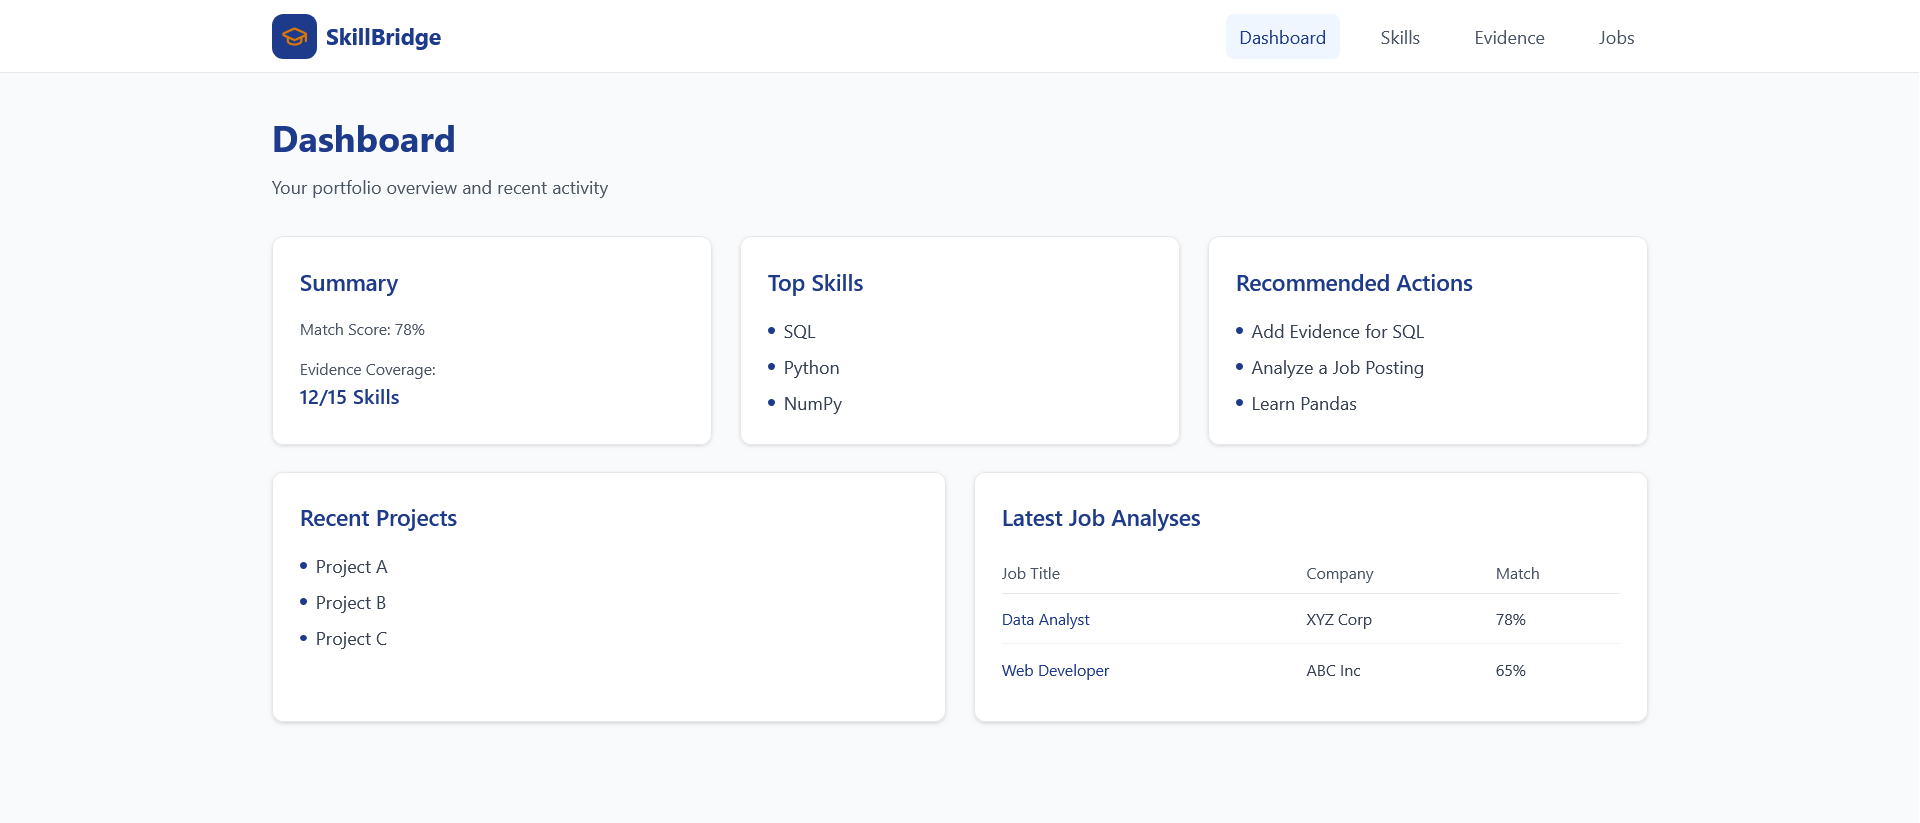
\includegraphics[width=\linewidth]{images/Dashboard.png}};
            \begin{scope}[x={(image.south east)},y={(image.north west)}]
                \node [anchor=south east, fill=black, fill opacity=0.5, text=white, font=\sffamily\tiny, inner sep=2pt, rounded corners=1pt] at (0.98, 0.05) {Dashboard View};
            \end{scope}
        \end{tikzpicture}
        \caption{Dashboard}
    \end{subfigure}
    \hfill
    \begin{subfigure}{0.48\textwidth}
        \centering
        \begin{tikzpicture}
            \node[anchor=south west, inner sep=0] (image) at (0,0) {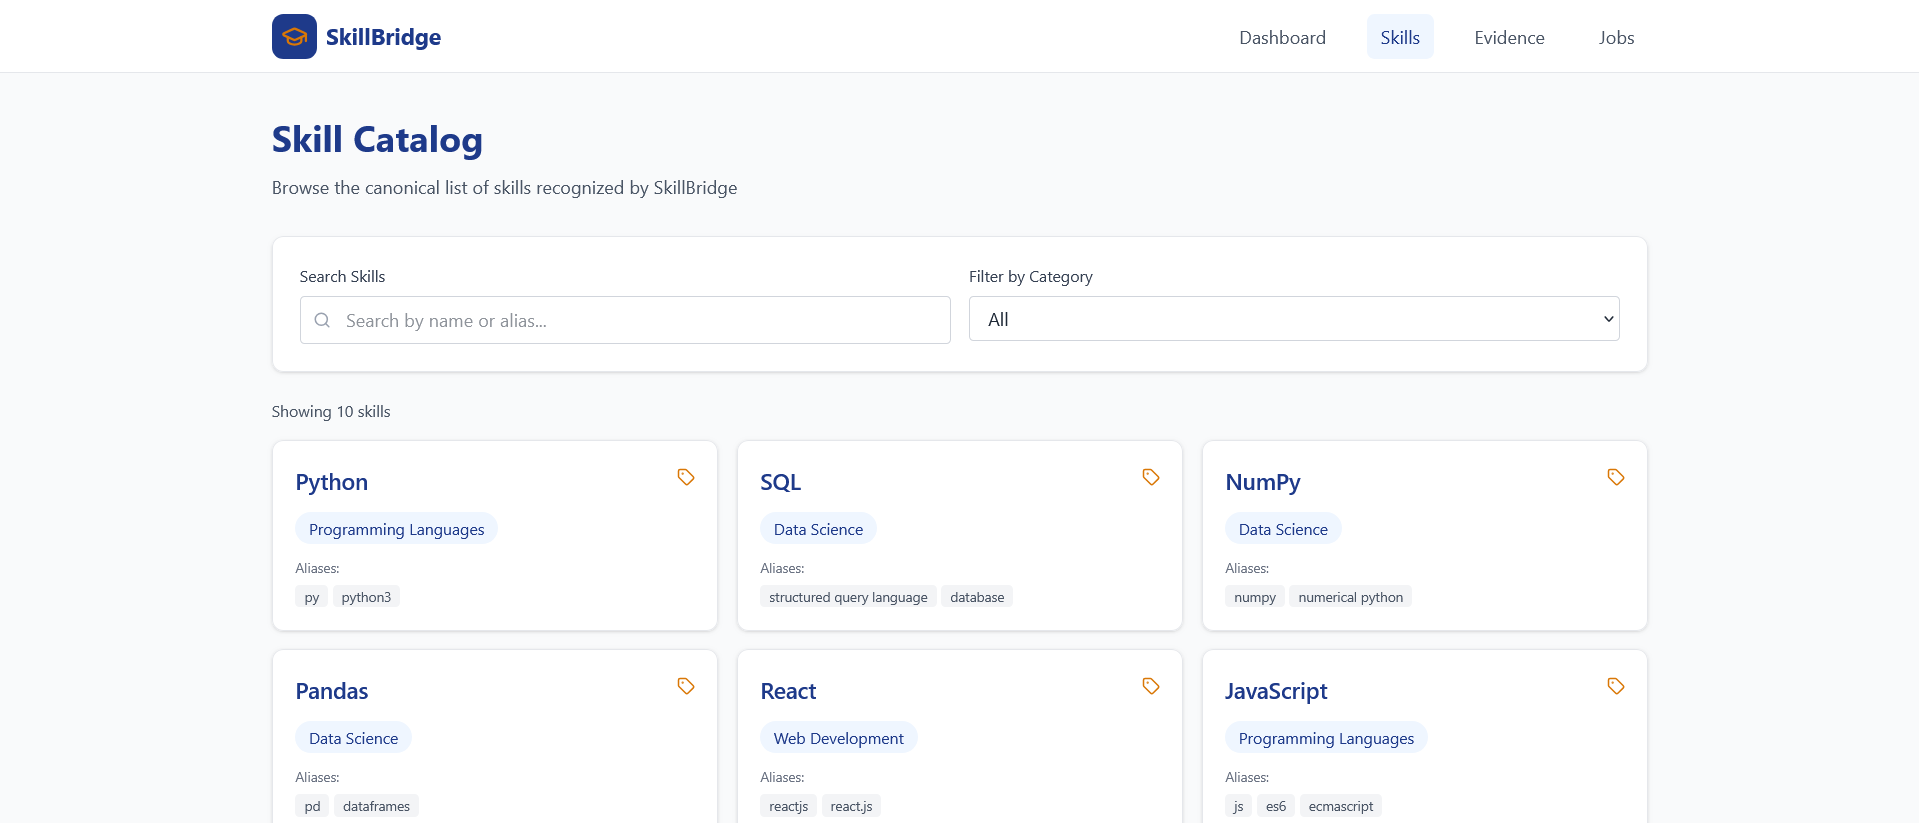
\includegraphics[width=\linewidth]{images/Skills.png}};
            \begin{scope}[x={(image.south east)},y={(image.north west)}]
                \node [anchor=south east, fill=black, fill opacity=0.5, text=white, font=\sffamily\tiny, inner sep=2pt, rounded corners=1pt] at (0.98, 0.05) {Skills View};
            \end{scope}
        \end{tikzpicture}
        \caption{Skills}
    \end{subfigure}

    \vspace{1em} % Space between rows

    % --- SECOND ROW ---
    \begin{subfigure}{0.48\textwidth}
        \centering
        \begin{tikzpicture}
            \node[anchor=south west, inner sep=0] (image) at (0,0) {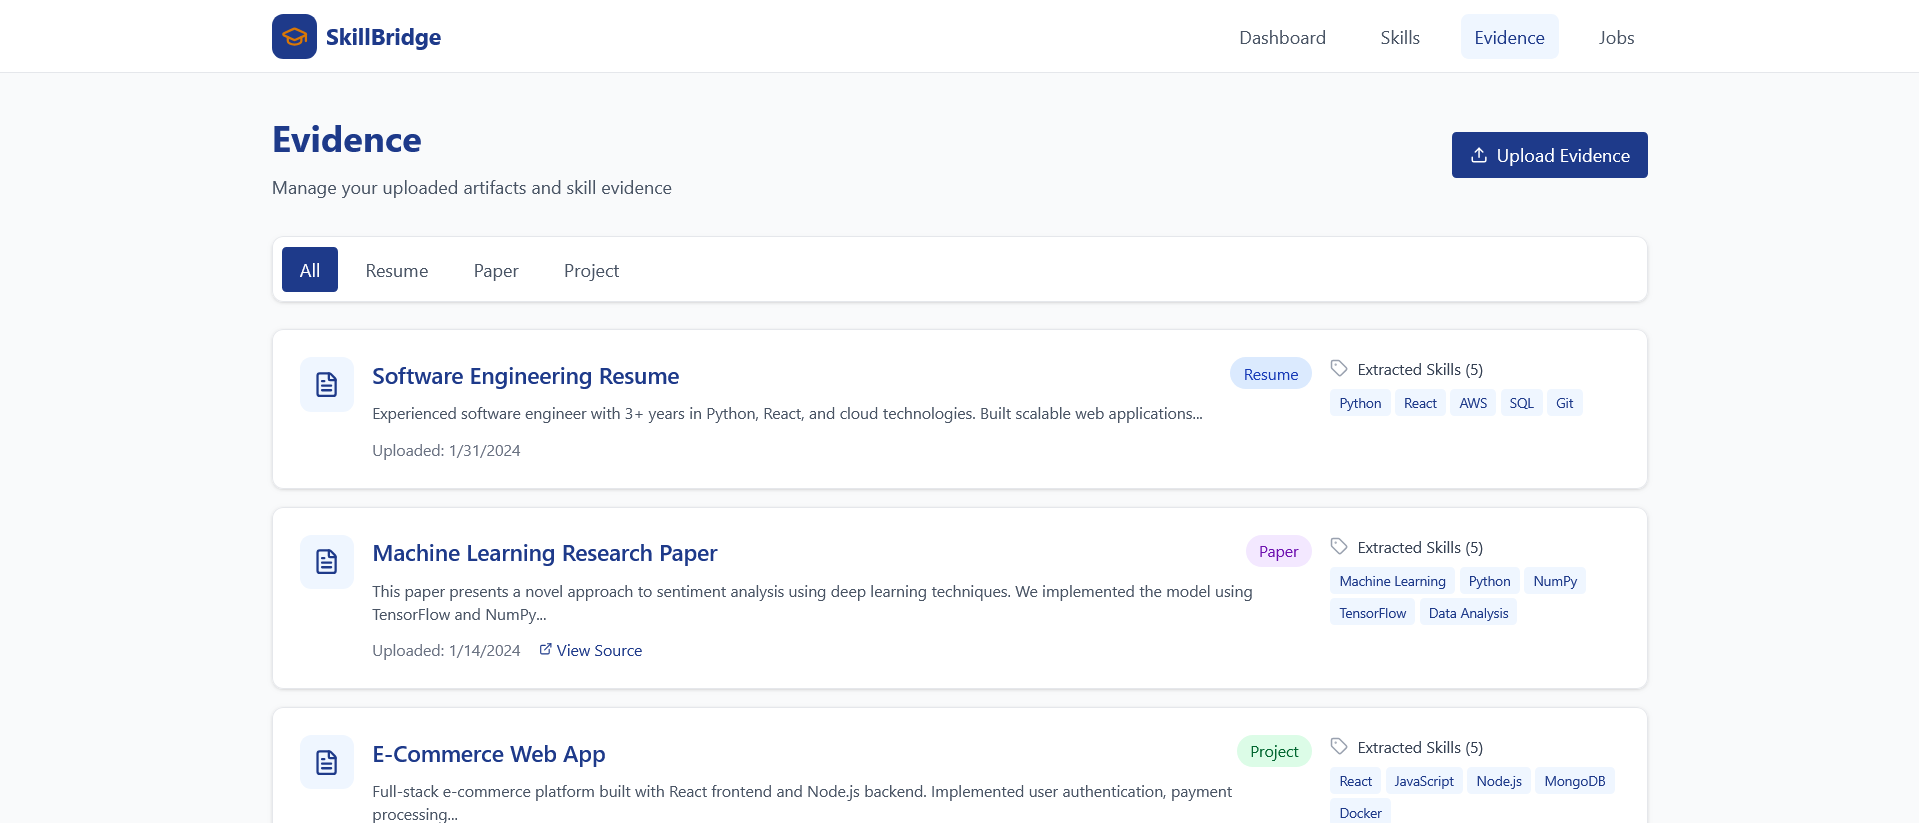
\includegraphics[width=\linewidth]{images/Evidence.png}};
            \begin{scope}[x={(image.south east)},y={(image.north west)}]
                \node [anchor=south east, fill=black, fill opacity=0.5, text=white, font=\sffamily\tiny, inner sep=2pt, rounded corners=1pt] at (0.98, 0.05) {Evidence View};
            \end{scope}
        \end{tikzpicture}
        \caption{Evidence}
    \end{subfigure}
    \hfill
    \begin{subfigure}{0.48\textwidth}
        \centering
        \begin{tikzpicture}
            \node[anchor=south west, inner sep=0] (image) at (0,0) {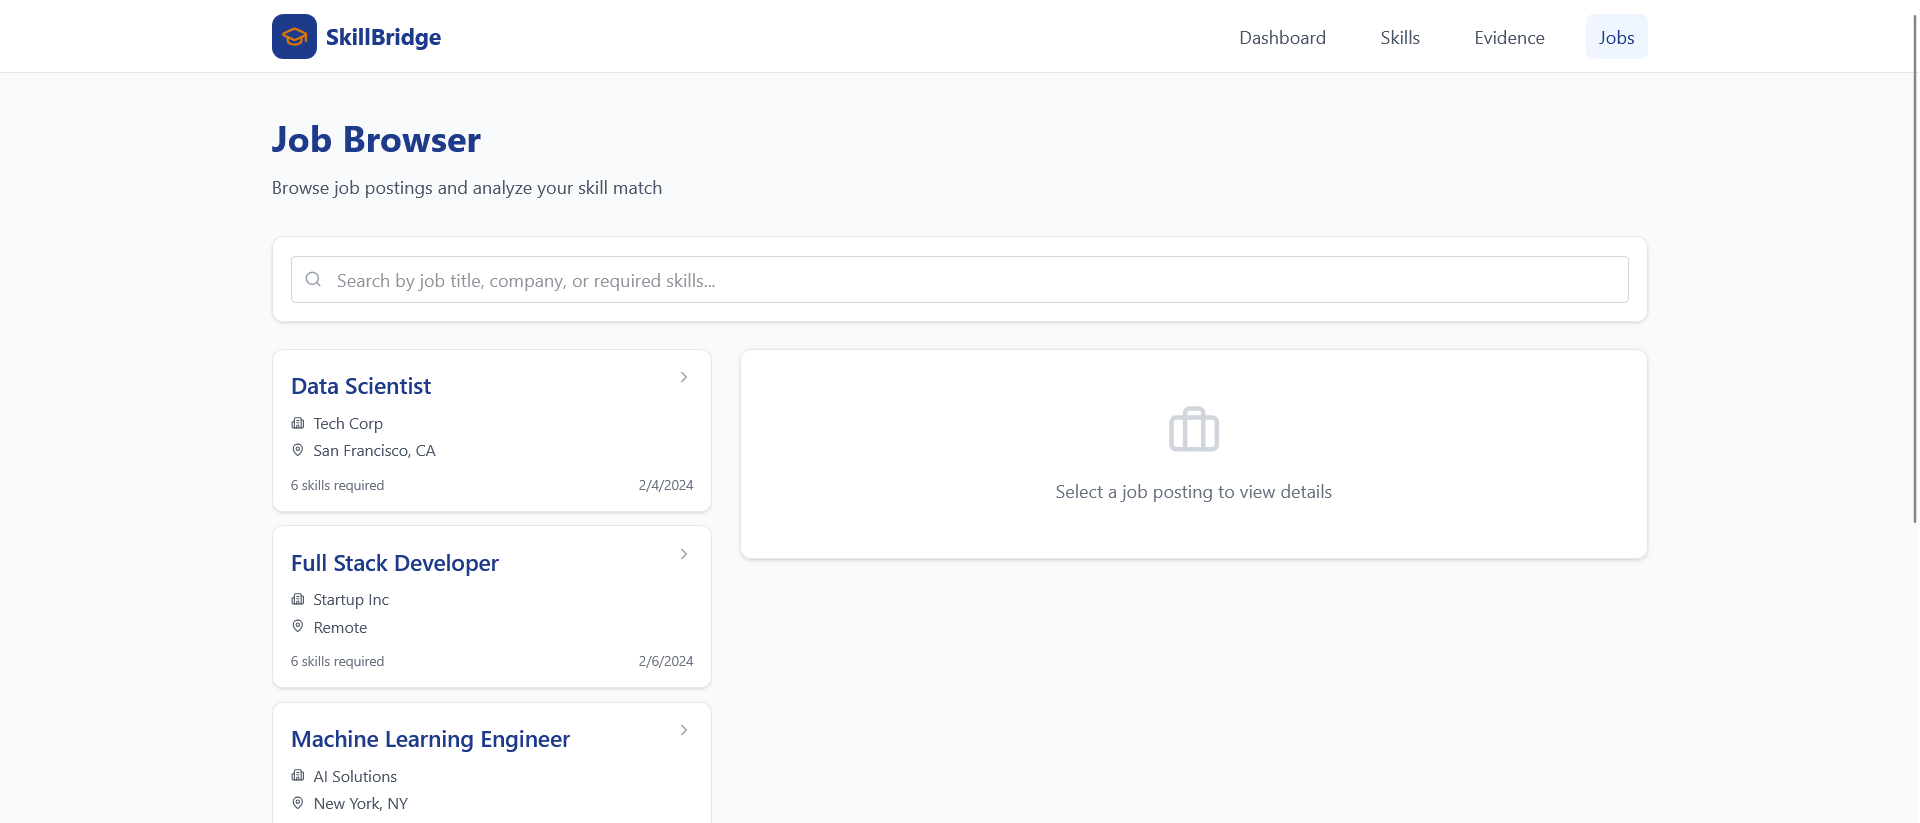
\includegraphics[width=\linewidth]{images/Job Browser.png}};
            \begin{scope}[x={(image.south east)},y={(image.north west)}]
                \node [anchor=south east, fill=black, fill opacity=0.5, text=white, font=\sffamily\tiny, inner sep=2pt, rounded corners=1pt] at (0.98, 0.05) {Job Browser View};
            \end{scope}
        \end{tikzpicture}
        \caption{Job Browser}
    \end{subfigure}

    \caption{Overview of the SkillBridge Platform interface modules.}
    \label{fig:skillbridge_ui}
\end{figure}

\subsection*{Week 1 -- How the UI Displays Data}

\begin{itemize}
    \item \textbf{Dashboard, The Overview:} The Dashboard acts as a command center, using individual summary widgets to display diverse data types: Key Metrics: Large-font text (e.g., "12/15 Skills") highlights critical progress. Lists: Simple bulleted lists display "Top Skills" and "Recommended Actions." Data Tables: The "Latest Job Analyses" section uses a traditional row-based table to compare specific data points like company names and match percentages.
    \item \textbf{Skill Catalog, Categorized Grids:} The "Skills" page presents information in a responsive grid of cards. Each card is standardized with: Category Tags: Colored labels (e.g., "Data Science") to define the skill's domain. Metadata Aliases: Smaller tags at the bottom of the card showing related search terms or versions (like "py" or "python3").
    \item \textbf{Evidence, Sequential Grids:} The Evidence section displays data as a vertical list of itemized cards. This allows for more detailed descriptions of specific files: Type Labels: Color-coded badges (Resume, Paper, Project) quickly identify the source of the data. Extracted Tags: Horizontal pill tags visualize the specific skills the system has pulled from each uploaded artifact.
    \item \textbf{Job Browser, Master-Detail Pattern:} The "Jobs" interface uses a split-pane layout common in productivity apps: Master List (Left): Concise preview cards showing the job title, company, and location. Detail View (Right): A larger space that expands when a card is selected, providing deeper data like specific skill requirements and an "Analyze Match" call-to-action.
\end{itemize}

% -------------------------
% Week 1 Images (DB screenshots + UI mockups)
% Replace filenames with your actual image paths.
% -------------------------

% DB screenshots (example: 2-up page)
% \MultiImagePageTwo{1}{images/week1_db_skills.png}{MongoDB: skills collection (sample documents)}
%                     {images/week1_db_jobs.png}{MongoDB: jobs collection (sample documents)}
%                     {Database Screenshots}

% Evidence + another DB view (example: 2-up page)
% \MultiImagePageTwo{1}{images/week1_db_evidence.png}{MongoDB: evidence collection (sample documents)}
%                     {images/week1_swagger_docs.png}{FastAPI Swagger (/docs) showing endpoints}
%                     {Database + API Screenshots}

% UI mockups (example: 4-up page)
% \MultiImagePageFour{UI Mockups (Planned Use Cases)}{images/week1_ui_skill_catalog.png}{UI Mockup: Skill Catalog}
%                      {images/week1_ui_evidence.png}{UI Mockup: Evidence Management}
%                      {images/week1_ui_jobs.png}{UI Mockup: Job Browser}
%                      {images/week1_ui_match.png}{UI Mockup: Match Results}

\end{document}
